\chapter{Introduction} \label{ch:intro}

\begin{figure}[h]
    \centering
    \begin{subfigure}{\textwidth}
    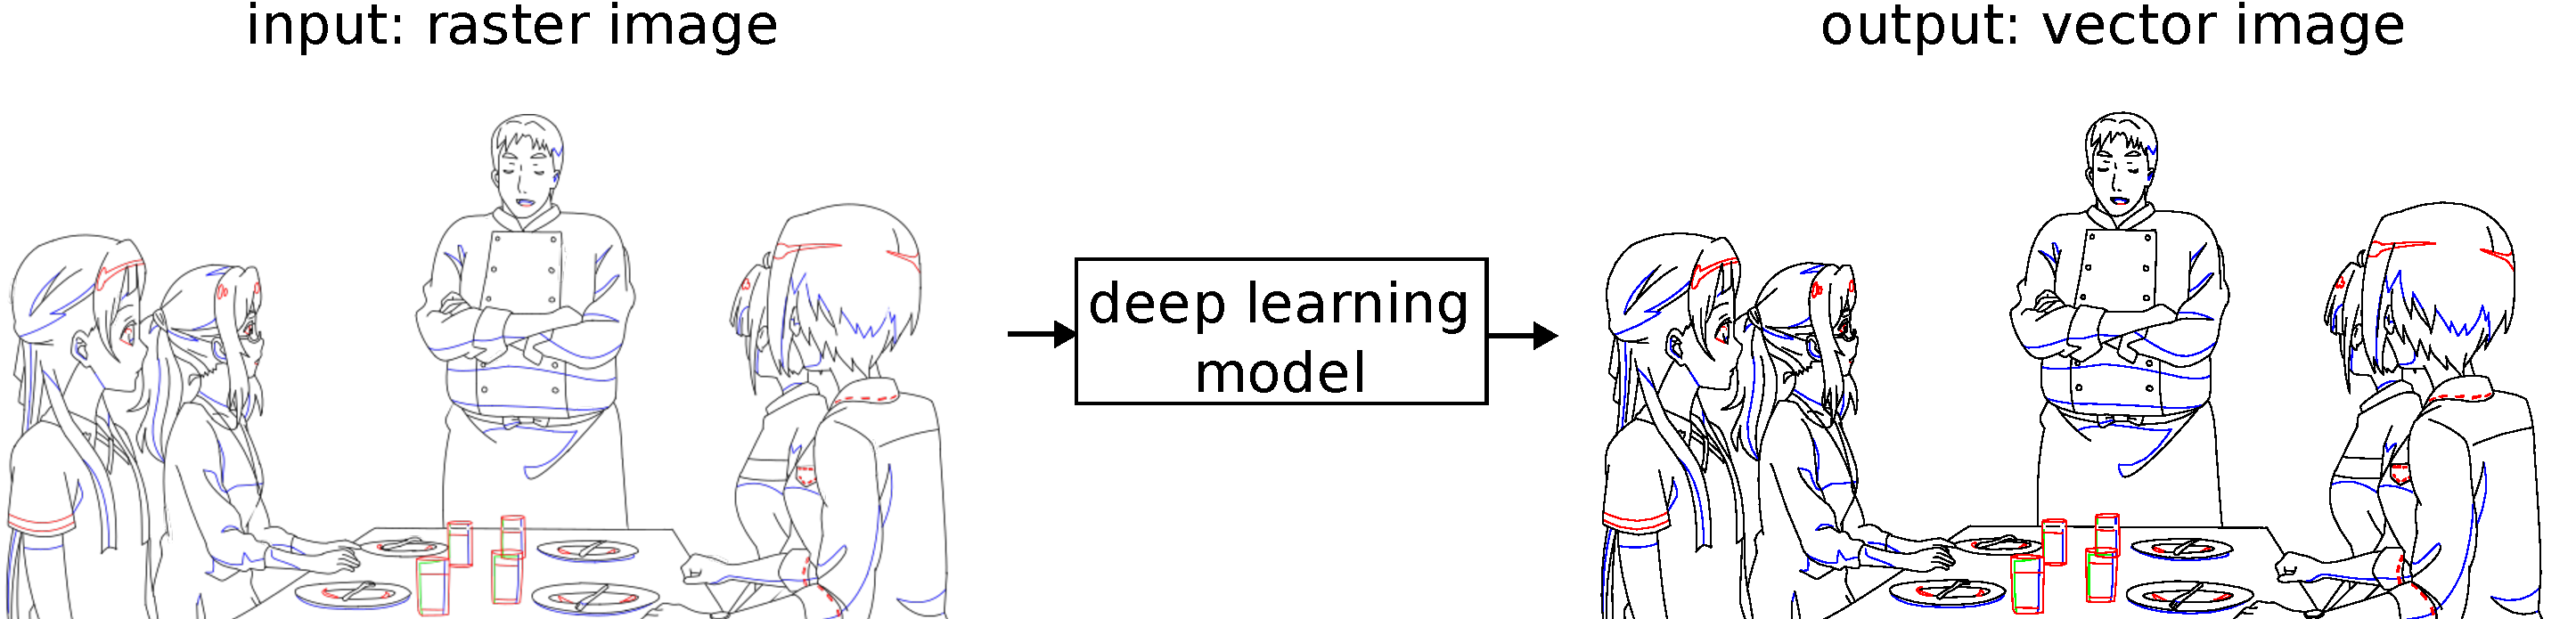
\includegraphics[width=\textwidth]{graphics/work_overview.pdf}
    \caption{The general design of the proposed objective. Input and output images are provided by Tonari Animation.}
    \end{subfigure}
    \begin{subfigure}{\textwidth}
    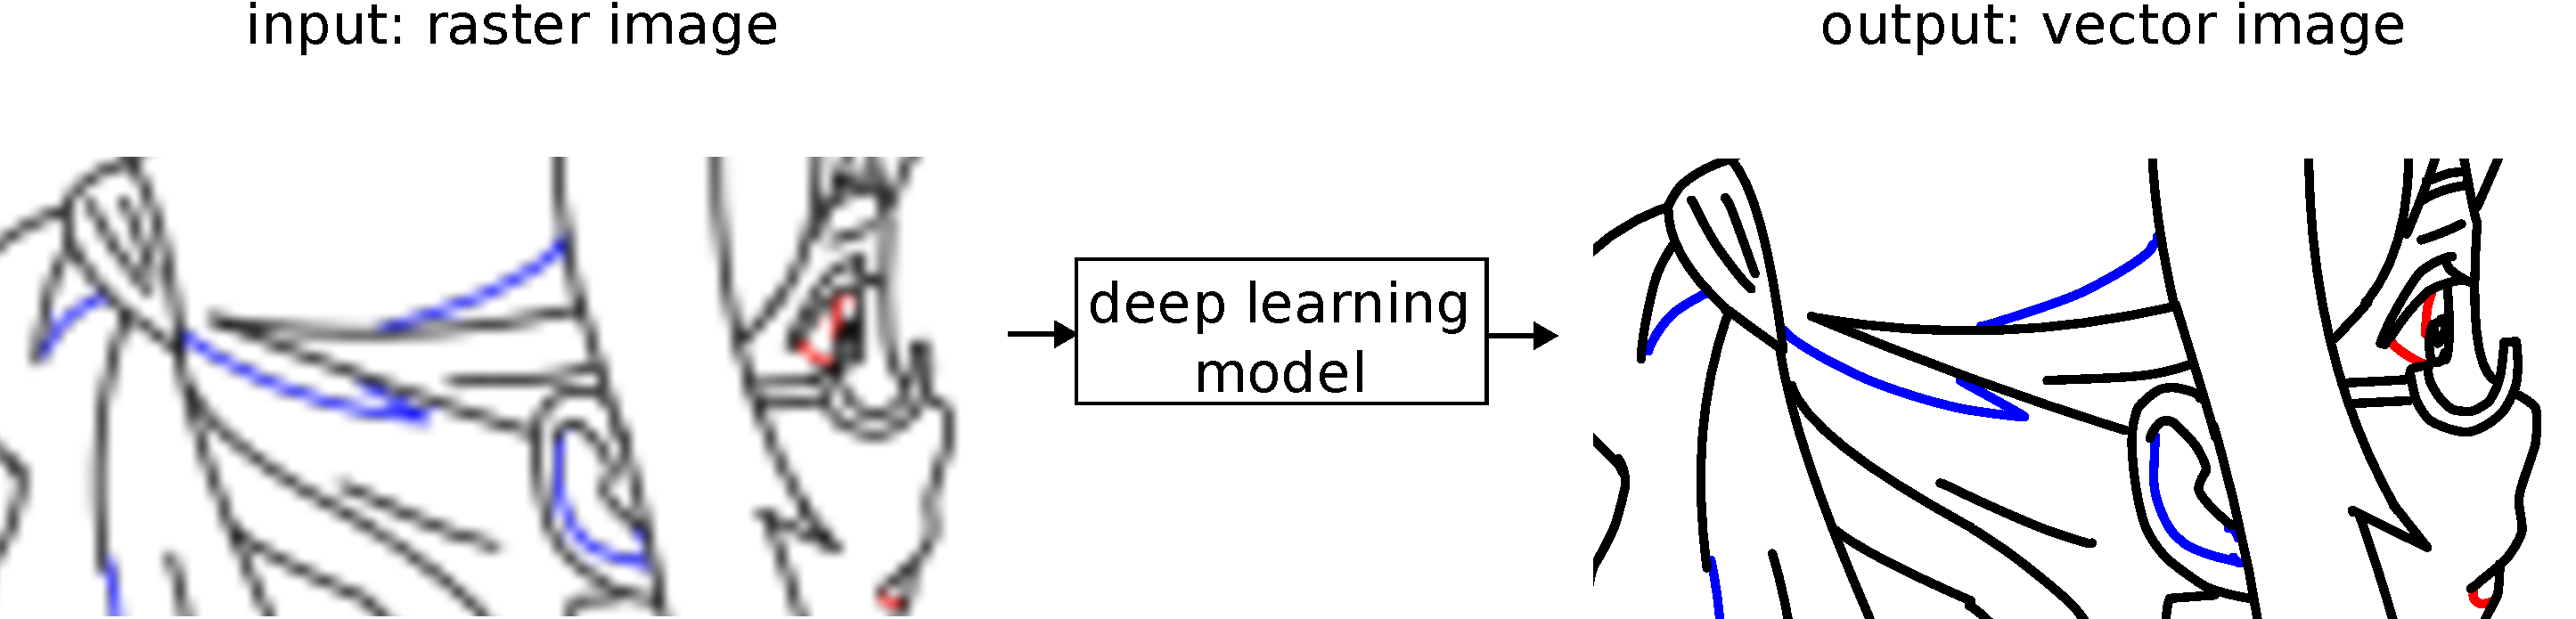
\includegraphics[width=\textwidth]{graphics/work_overview_zoom_8x.pdf}
    \caption{Highlighted section of input and output images, which reveals structural differences.}
    \end{subfigure}
    \caption{Overview of the research objective. The objective is to automatically convert clean animation frame line-art raster images into vector images. Zooming into the figure reveals the structural difference between the input and the output image. Note that the output image is taken from the gold standard test dataset. For a genuine reconstruction result of the developed line-art vectorization method, refer to \Cref{fig:input.output.example}}
    \label{fig:work-overview}
\end{figure}

In principle, animation consists of sequentially showing single frames in order to achieve the visual effect of a moving scene. \emph{Limited animation} is an animation technique in which frames are not completely redrawn (like in full animation), but where the moving parts (also called \emph{cels}) are reused over frames. While both full animation and limited animation techniques reuse some fixed parts (like the background), the reusing of cels by limited animation leads to the characteristic stiff style and reduces the cost to produce an animated series. Today, the technique is primarily used in hand-drawn animations, often under the term \emph{anime} popularized by Japanese media.

While limited animation was mostly replaced with full animation and 3D animation in the western world, it still enjoys continued relevance due to the growing importance of anime. This importance is underlined by \citet{napier2016anime}, who estimates that anime made up over 60 percent of all animated shows in 2016. Unsurprisingly, anime is especially prevalent in Japan, where it accounts for 6 of the top 10 highest-grossing films in 2021 \citep{jpboxoffice}. According to \citet{animeindustryreport}, the worldwide market for anime monotonically grew from 1266.1 billion Yen in 2009 to 2742.5 billion Yen in 2021 (with an exception in the year 2020). This trend suggests that limited animation will continue to be relevant in the future.

The hand-drawn limited-animation production process is composed of four phases. Based on the storyboard produced in the first phase, animators repeatedly draw and improve rough key frames in the second phase. These keyframes are line drawings only drawn for critical moments in a scene and contain mostly cels. In the third phase, the keyframes are vectorized and cleaned. To achieve the visual effect of fluidity, a large number of frames in between the keyframes are drawn. In contrast to full animation, these \emph{inbetweens} are not redrawn completely, but reuse the majority of a keyframe while only editing small parts of the image. Finally, in the fourth phase, the clean frames are colored and enriched with special effects and a background image.

Thus, the production consists of creative parts such as the drawing of keyframes and tedious tasks such as the creation of inbetweens. The latter tasks are a ripe target for automatization, freeing up animation studios to focus on the creative parts of their work. This work explores the automatization of one such task, specifically the vectorization of clean animation frames.

Traditionally, computational tasks are automated using hand-crafted algorithms with manually set parameters. While this is feasible for well-defined and structured tasks, it is unfeasible for complex, ambiguous tasks with high-dimensional data, such as the vectorization of clean animation frames. A different automatization technique that is better fit for these types of tasks is \emph{machine learning}. Contrary to hand-crafted algorithms, machine learning consists of assembling a large dataset of inputs and outputs and defining an algorithm which exploits statistical correlations in this dataset to fit a model that generalizes to data outside of this dataset. A subset of machine learning that has increased in importance in recent years is \emph{deep learning}, in which the model fit to the dataset is an artificial neural network \citep{Rosenblatt58theperceptron}.

In this chapter, \Cref{sec:motivation} provides the motivation for the research. 
\Cref{sec:intro.problem} details the research question and related research objectives. \Cref{sec:challenges} lists the challenges associated with the research objectives. \Cref{sec:intro.goals} gives a summary of the main contributions of this work. Finally, \Cref{sec:intro.structure} outlines the structure of the thesis.

\section{Motivation}
\label{sec:motivation}
%Hand-drawn animation could greatly benefit from machine learning methods, but there are little publicly known success stories. \josh{elaborate the rest of this paragraph bit more} Yet, very little work using machine learning on hand-drawn animation production exists, and existing work focuses on models that operate on final video frames. This comes in clear contrast with research on illustration and comics, for which a lot more research exists.

In order for the limited animation production process to proceed as quickly and as accurately as possible, clean frames need to be drawn as vector images. Contrary to raster images, which represent an image using a raster of color values, vector images represent an image using a hierarchy of graphical primitives. The primitives used in this case are lines and curves. Having the clean frame as vector line art enables accurate and easy editing. Furthermore, vector files are resolution-independent and require less data to represent an image than lossless raster formats, where the color of each pixel needs to be stored somehow. Moreover, by their nature they also contain the semantic composition of the image, which is potentially useful for downstream tasks.

In many animation studios, limited animation frames are initially drawn on paper, i.e., in raster format. Afterwards, these frames need to be manually traced in order to produce clean frames in vector format. This manual conversion is a tedious and time-intensive process, requiring roughly an hour per frame. Hence, it would be beneficial to have a method which can convert the clean frame into vector format automatically.

Even disregarding the step from rough animation frames in raster format to clean frames in vector format, there are scenarios where the clean frame is only available as a raster image. This could be due to various reasons, including discontinuity in the production workflow (e.g., when different studios are contracted for different steps), the need to export an image from the drawing program to another application, or the existence of old production data that needs to be reused.

Once the clean animation frame is available in vector format, it increases the efficiency of successive workflow steps. An example is the creation of the frames inbetween keyframes, where artists can naturally utilize existing keyframes and only edit a small part of the image. As an example, the curves making up strains of hair could simply be moved instead of needing to be completely redrawn in the case of a raster image.

In summary, in the event of clean animation frames being only available in raster format, it is necessary to manually vectorize the images before they can be used efficiently. Therefore, this work explores the possibility of automatizing this laborious process using line-art image vectorization methods. 

\section{Aim of the Work}
\label{sec:intro.problem}

The purpose of this work is to create a method to automatically convert clean animation frame raster images into corresponding vector images. As mentioned in \Cref{fig:work-overview}, this method consists of a deep learning model trained on clean animation frames. For the resulting line-art vector image to be useful for artistic purposes, the content needs to be semantically meaningful, i.e., the arrangement, topology and parameterization of graphical primitives (i.e., lines and curves) need to make sense and be close to how artists would draw. This prevents traditional algorithms \citep{Selinger03potrace:a, autotrace, 10.1145/2421636.2421640} to be used for that purpose, as these often produce vector images that visually resemble the raster image closely, but contain semantically meaningless vector primitives - for example, a naive but visually convincing vectorization solution is to represent each pixel as a small line.

In detail, this work will attempt to answer a \paragraph{\gls{rq1}}, which is to what extent is it possible to automatically vectorize clean animation frame line art in a manner that is semantically meaningful?

\section{Challenges}
\label{sec:challenges}

Creating the deep learning-based method to vectorize clean animation frames represents a challenge in itself, due to the visual structure of the images. Specifically, it is crucial that the output of the proposed deep learning model is structurally similar to real clean frame vector images, i.e., that the output consists solely of the primitives that artists use to draw clean animation frames. Hence, it is necessary to find a representation of these primitives that is suitable for deep learning models.

Another challenge is the low amount of available data. While a small dataset ($N=139$) of raster/vector image pairs of clean frames was provided to us as part of a research project (and drawn at the Tonari Animation studio), this is not a sufficient quantity to fit a deep learning model. Since there is little publicly available data for this task, extending the dataset is non-trivial. In order to achieve this, data augmentation methods have to be used in addition to procuring public data.

Moreover, clean animation frame images often contain a large amount of curves (usually more than 1000 lines per image). The proposed solution needs to be designed in a way to handle this large amount of primitives, since prior deep learning-based works are often suited only for images with a lower amount of curves. 
Additionally, it is necessary for the image vectorization method to be applicable at lower image resolutions, since clean frame raster images (especially older production data) are often at a resolution for which existing algorithms were not designed.
Furthermore, it is unavoidable that the resulting vector images will contain errors and therefore need to be corrected manually. Hence, the solution should focus more on getting the curves it generates correct, rather than covering all curves in the input image. In other words, a solution that generates half of the curves completely correct is preferable to a solution that generates all of the curves only somewhat correct, since in the latter case all curves have to be manually corrected anyway.

Finally, the clean animation frame vectorization method should be designed as a deep learning model, as this makes it easier to adapt it to vectorize raster images from different domains using finetuning. This is important for a related task, which is motivated in the following: One factor that has greatly limited successful attempts in the field of deep learning in hand-drawn limited animation production is the scarce amount of available production data that can be used for training. While it is probably fruitless to attempt to design a system that generates the whole animation automatically, solving individual steps in the production process might be possible. It is clear that training such models would require a large amount of production data, specifically production data that is in reverse order of the actual production workflow. As an example, if a large dataset of clean keyframes and associated inbetweens (as well as animation timesheets) was available, it would be possible to train an inbetween generation model. Other potential uses include clean frame coloring, inpainting or compositing.

While the obvious way of attaining an animation production dataset would be for a studio to publish it, thus far no such dataset has been published, which presents another challenge. An alternative would be to synthesize the data. The differentiable nature of the proposed line-art vectorization algorithm could be utilized for that purpose. While the model will be trained using clean frames as input data, it might be possible to extend or finetune the model to use images of another domain (such as final animation frames) as input. Then, it could be used for a cross-domain vectorization model in order to convert raster images of one domain (e.g., final animation frames) into vector images of another domain (i.e., clean frames). \Cref{fig:cross-domain-overview} depicts such a model. Since final animation frames are readily available in high quantity and quality, this would potentially make it possible to synthesize a large dataset of clean frames requiring only small supervision. However, creating such a model is not the focus of this work, rather, the above-mentioned line-art vectorization method is designed in a way such that it could in principle be extended to cross-domain line-art vectorization. Most importantly, this means that the model is nearly end-to-end differentiable, such that it can be easily finetuned on other data. This is a characteristic that traditional algorithms \citep{Selinger03potrace:a, autotrace, 10.1145/2421636.2421640} do not possess.

In summary, the quantity of the data and the qualitative structure of the data domain impose a range of restrictions which need to be accounted for in the architecture design of the method. Furthermore, the method should be based on a deep learning model in order to enable adaptability to other input data domains.

\begin{figure}
    \centering
    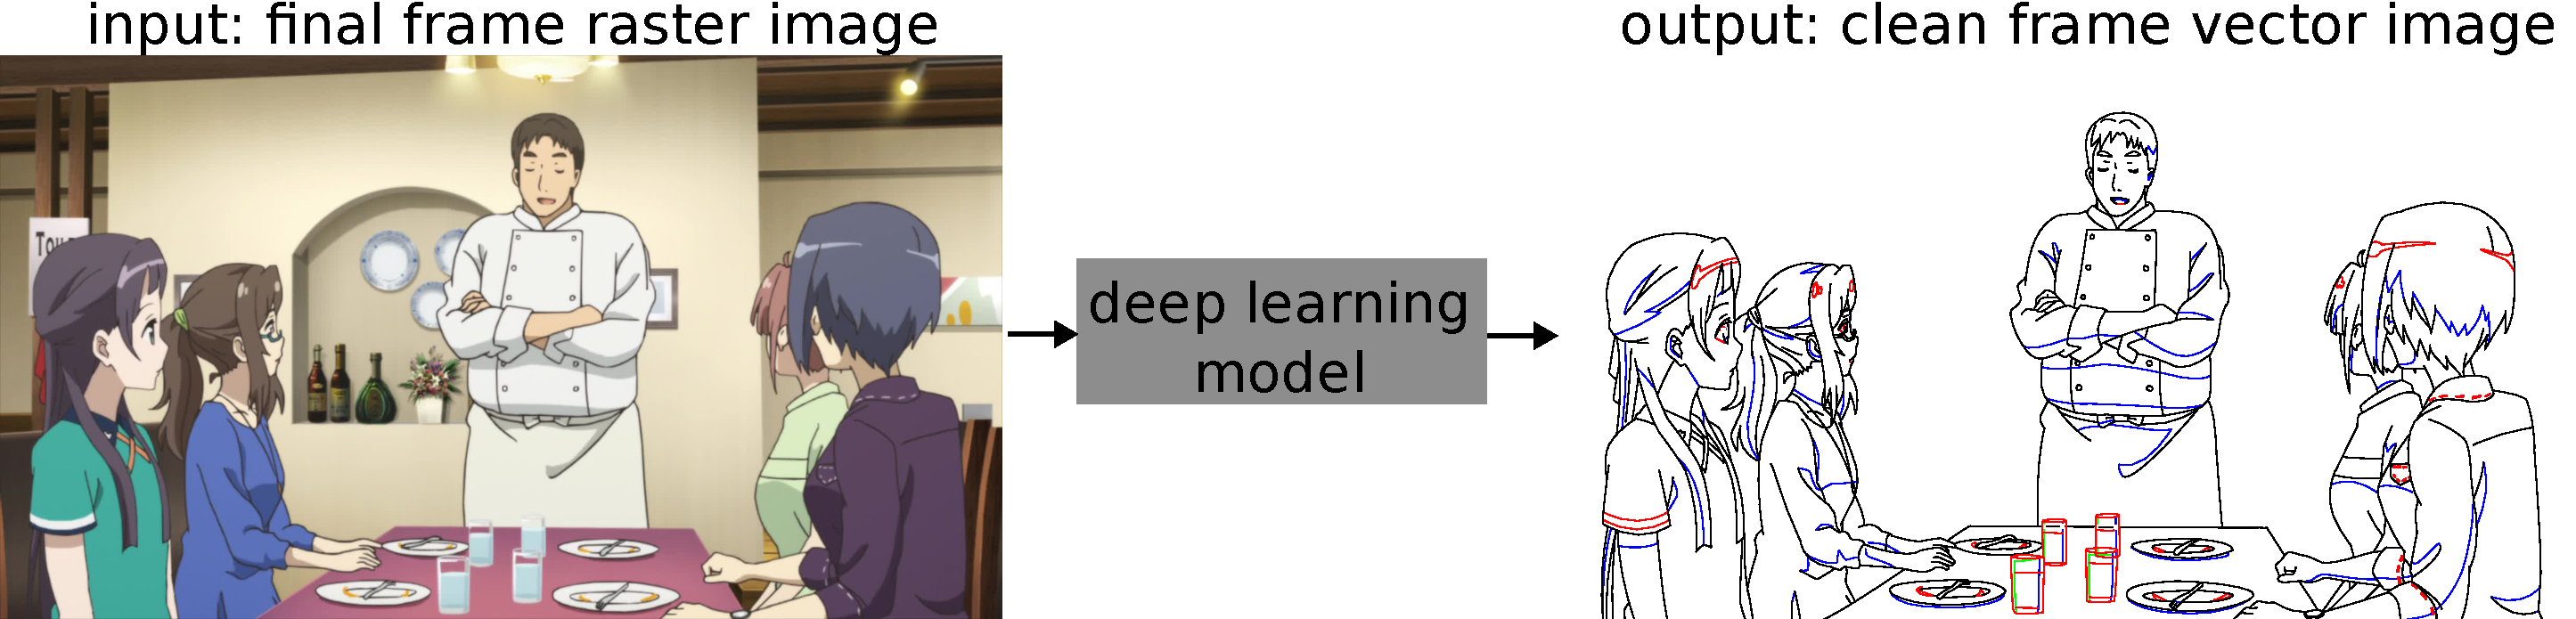
\includegraphics[width=\textwidth]{graphics/cross-domain-overview.pdf}
    \caption{An overview of cross-domain line-art vectorization, a potential extension of the proposed solution. Here, the objective is to convert final animation frame raster images (example by \citet{sakura-quest}) into clean animation frame vector images by extending or finetuning the deep learning model depicted in \Cref{fig:work-overview}.}
    \label{fig:cross-domain-overview}
\end{figure}

\section{Contributions}
\label{sec:intro.goals}

To answer \gls{rq1}, the \gls{ro1} is to create a method for line-art vectorization that takes clean animation frame raster images as input and outputs the corresponding semantically meaningful vector image. This method is described in \Cref{sec:model} and based on a deep learning model to enable it to be adapted to different input image domains. Furthermore, it is designed to fit the qualitative structure of clean animation frames as input and output images. 

Accordingly, the \gls{ro2} is to perform an evaluation that ascertains the extent to which the developed method and existing state-of-the-art line-art image vectorization methods are able to vectorize clean animation frames. This evaluation is described in \Cref{sec:eval}. Great care is taken to ensure that this evaluation is reproducible. Due to this, the whole evaluation is not only conducted on the clean animation frames provided by Tonari Animation, but also on a publicly available subset of the SketchBench \citep{Yan:2020:ABR} dataset. Furthermore, the code for the evaluation is publicly available at \url{https://github.com/nopperl/marked-lineart-vectorization}. Ultimately, while the evaluation shows advantages of the developed line-art image vectorization method compared to existing state-of-the-art methods, no method is able to satisfactorily vectorize clean animation frames.

\paragraph{\gls{ro1}} A deep learning-based method for clean animation line-art vectorization.
\paragraph{\gls{ro2}} A reproducible evaluation assessing the extent to which line-art image vectorization methods can vectorize clean animation frames.

\section{Structure}
\label{sec:intro.structure}

\Cref{ch:bg} describes the necessary prerequisites required to understand the proposed solution. \Cref{ch:related} gives an overview of prior work related to the research objectives. The proposed solution is described and empirically evaluated together with state-of-the-art methods in \Cref{ch:alg}. \Cref{ch:conclusio} revisits the research objectives, lists limitations and provides potential future work.
